\chapter{GTFS}
\label{2-teorie-gtfs}

General Transit Feed Specification, zkráceně GTFS, je dokument, který definuje
obecný formát pro jízdní řády veřejné dopravy a příbuzné geografické informace.
GTFS „feeds“ umožňují veřejným dopravním agenturám zveřejňovat svá přepravní
data a vývojářům psát aplikace, které tato data spotřebovávají interoperabilním
způsobem. \cite{gtfs-info}

\section{Historie GTFS}
V Portlandu ve státě Oregon v USA se společnost TriMet pokusila jako jedna z prvních 
řešit problém s plánováním tranzitní dopravy pomocí otevřených dat sdílených širokou veřejností.
V roce 2005 společnost TriMet oslovila společnost Google s dotazem, zda mají nějaké plány
na začlenění tranzitní dopravy do svých plánovačů výletů na základě veřejných údajů TriMet.
Google jim kladně odpověděl a spojily síly s implementací jednoho z prvních plánovačů výletů v Portlandu.

Jedním z prvních problémů, kterým TriMet a Google čelily, byl problém udržitelných dat 
- pro zajištění kvalitních cest by plánovač cest potřeboval kvalitní přepravní řád, 
trasu a údaje o zastávkách v elektronickém formátu, který by byl neustále aktuální. 
Společnost TriMet ve spolupráci se společností Google naformátovala svá přepravní 
data do snadno udržovatelného a spotřebního formátu, který lze importovat do Map Google. 
Tento formát dat přepravy se stal známým jako Specifikace zdroje Google Transit (anglicky
Google Transit Feed Specification (GTFS)). 
V roce 2005 byla tato služba plánování cesty spuštěna jako Google Transit.

Od tohoto roku se GTFS stal nejpopulárnějším datovým formátem pro přepravní služby na světě. 
Spousta agentur se rozhodla sdílet své GTFS údaje s veřejností, zatímco některé agentury 
zůstaly zdrženlivé a přístup k datům nechaly jen některým partnerům. Ke 2. prosinci 2019
uvádí OpenMobilityData 1233 poskytovatelů s veřejně přístupnými kanály GTFS,
z nichž 465 je ve Spojených státech. 

V důsledku inovací vývojářů třetích stran jsou data GTFS nyní využívána různými softwarovými aplikacemi
třetích stran k mnoha různým účelům, včetně plánování výletů, map, vytváření jízdních řádů, mobilních dat,
vizualizace, přístupnosti, analytických nástrojů pro plánování a informační systémy v reálném čase.
V roce 2010 byl název formátu GTFS změněn na General Transit Feed Specification,
aby přesně reprezentoval jeho použití v mnoha různých aplikacích mimo produkty Google. \cite{transitwiki} 

% doplnit něco o historii GTFS 

\section{GTFS dataset}
GTFS dataset\footnote{kolekce dat, která by měla být publikována na permanantní URL adrese}
obsahuje CSV soubory, jehož úplný seznam je v následující tabulce. Co je to CSV soubor?

CSV, \textit{Comma-separated values}, v překladu \textit{hodnoty oddělené čárkami}, je jednoduchý 
souborový formát určený pro výměnu tabulkových dat. Data jsou oddělována „oddělovačem“.
Ačkoli podle definice by měl být formát oddělen čárkami, oddělovač může být prakticky cokoli. 
Nejčastějšími oddělovači jsou právě čárky, středníky nebo mezery. CSV soubor se 
může upravovat v jakémkoliv textovém editoru.
\begin{figure}[H] \centering
    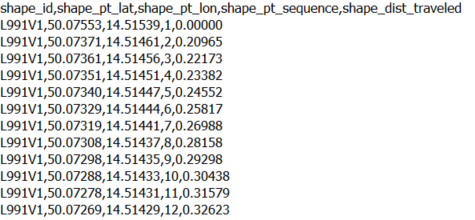
\includegraphics[width=250pt]{./pictures/ukazka-csv.PNG}
    \caption[Ukázka CSV formátu ze souboru shapes.txt]{Ukázka CSV formátu ze souboru shapes.txt}
	\label{fig:ukazka-csv}              
\end{figure}
V GTFS datasetu je určité množství povinných a nepovinných CSV souborů v textové podobě.
 

Tučně zvýrazněné pole jsou požadované či podmíněně vyžadované. Ostatní pole jsou 
volitelné. 
\begin{figure}[H] \centering
    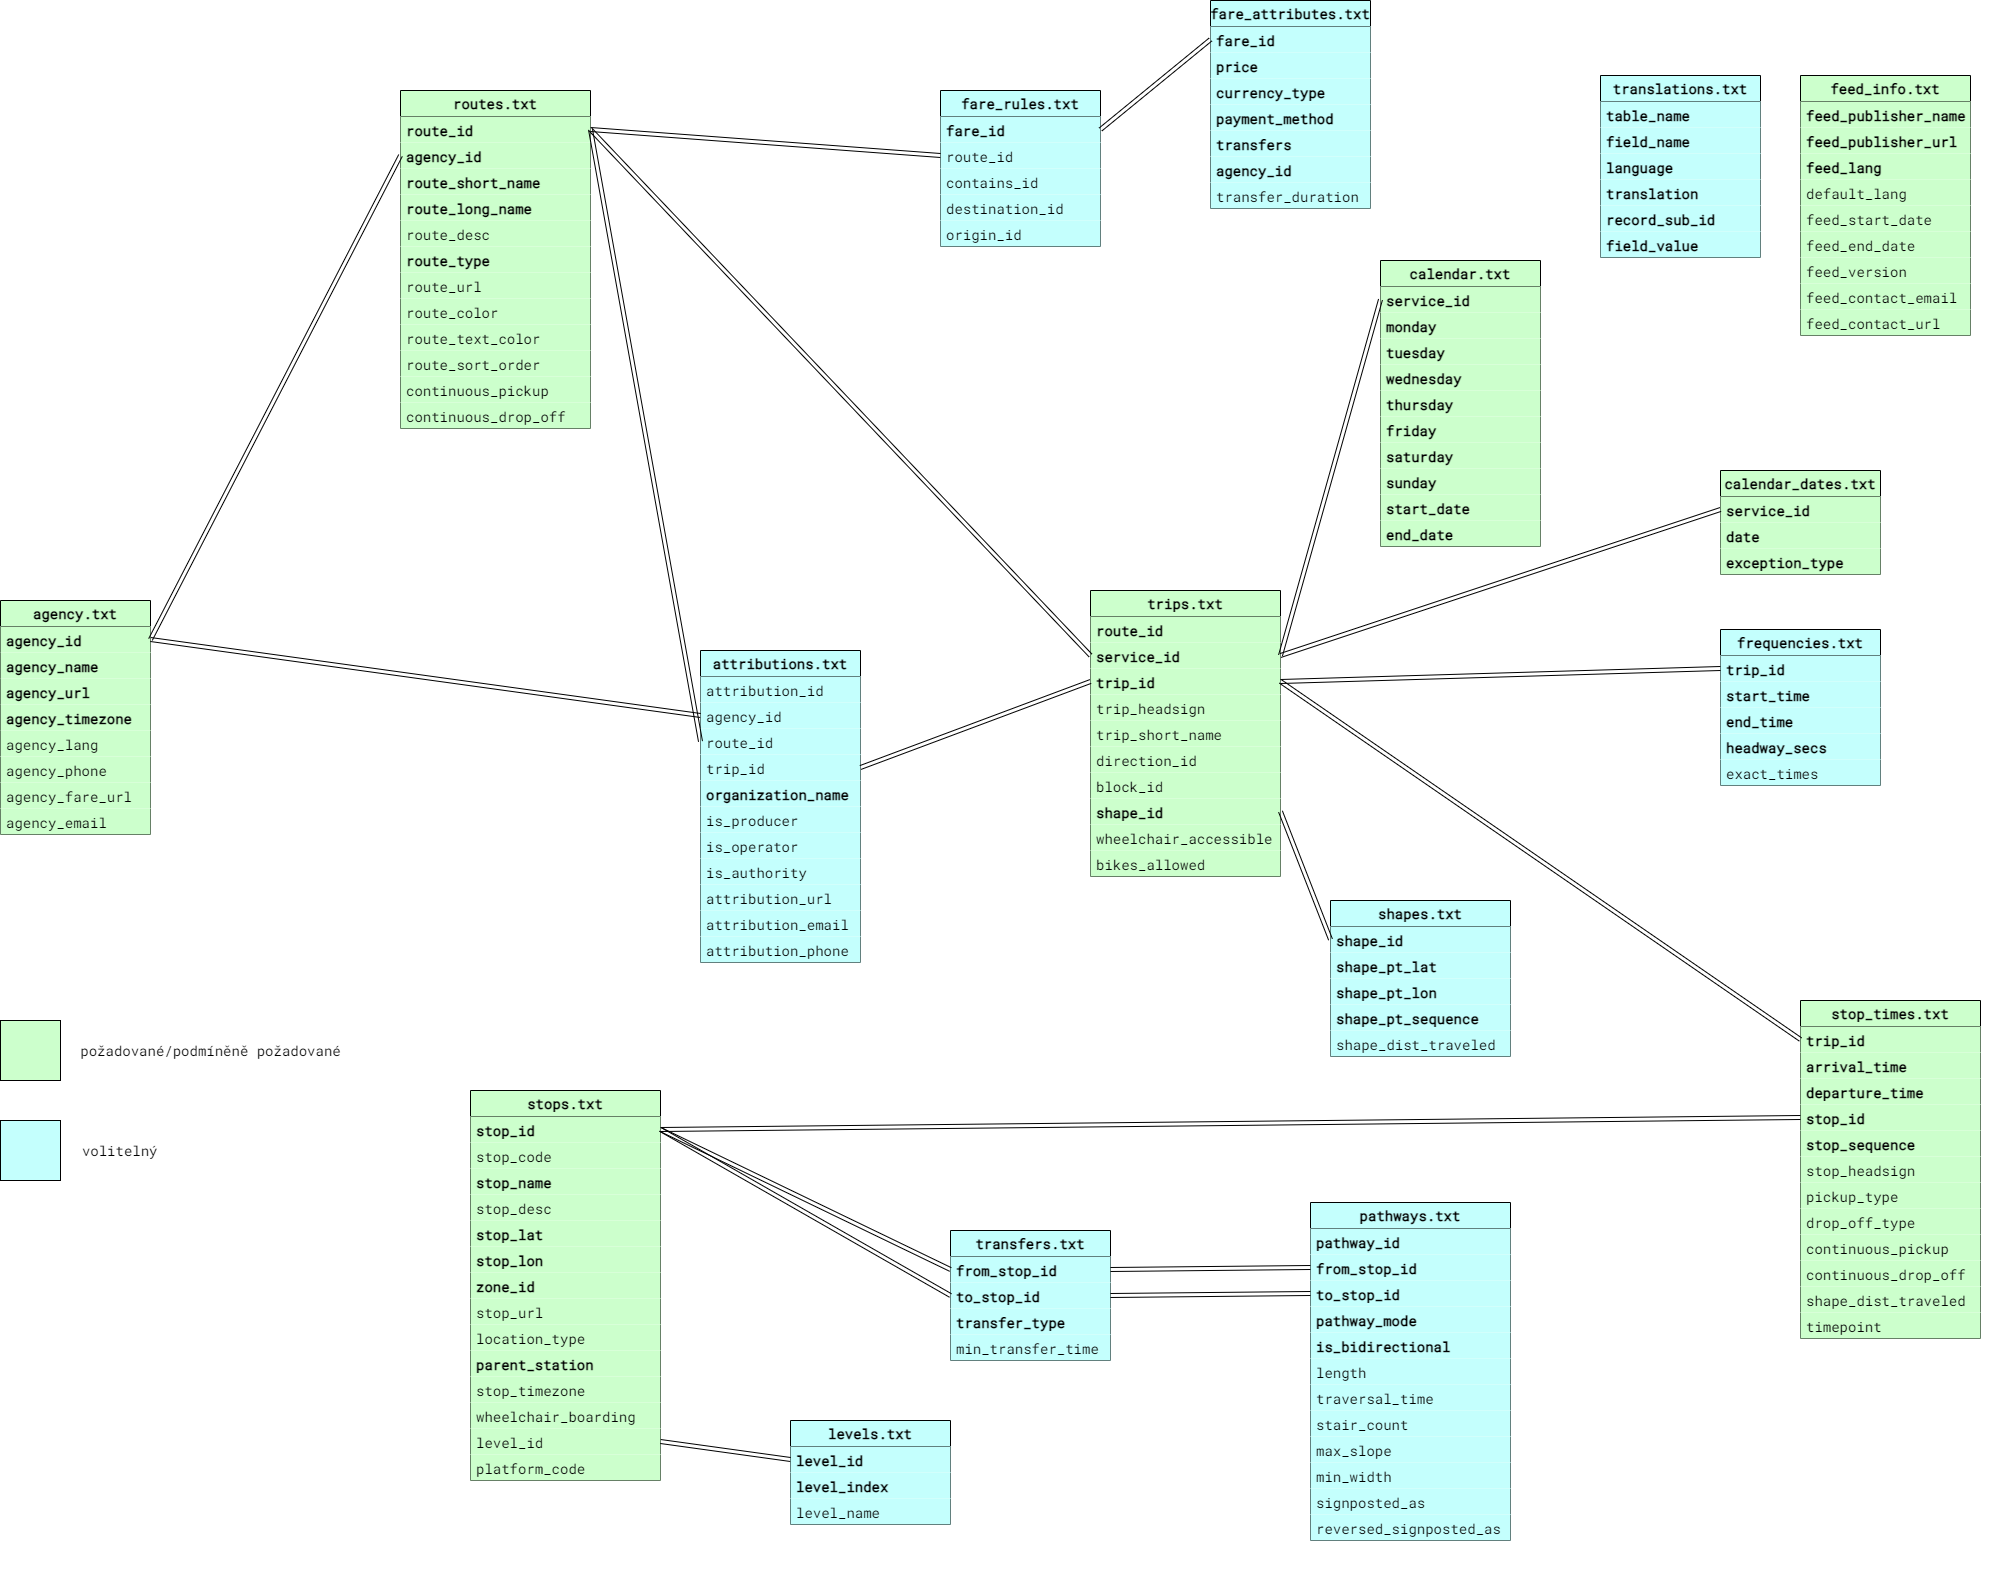
\includegraphics[width=400pt]{./pictures/GTFS-diagram.PNG}
    \caption[Diagram GTFS datasetu]{Diagram GTFS datasetu}
	\label{fig:GTFS-diagram}              
\end{figure}
